
\subsection{Introduction to convex optimization problems}
General form: Consider the functions $F_i(x), h_i(x): \reals^n\rightarrow \reals$.
\begin{align*}
\min_{x\in \reals^n} \quad &F_0(x) \quad \text{"objective function"}\\
s.t. \quad &F_i(x) \leq 0, i = 1...m \quad\text{inequality constraints}\\
&h_i(x) =0,i =1...p \quad \text{equality constraints}
\end{align*}


Feasible set for this question:
$$\mathcal{C} = \{x\vert F_i(x) \leq 0,i=1...m,h_i(x) = 0,i = 1...p \}$$


Optimal value: $p^* = \inf_{x\in \mathcal{C}}F_0(x)$. Note that it could be $\infty$, and also could be empty.

Optimal points: $\{x\in \mathcal{C}\vert F_0(x) = p^* \}$. Note that it could be empty, and also could be not unique.



\begin{example}
Consider the optimization problem:
\begin{align*}
\min_x \quad &\min x_1 + x_2 \\
s.t. 
&-x_1\leq 0\\
&-x_2\leq 0\\
&1- x_1 x_2\leq 0\\
\end{align*}

So $x^*=
\begin{bmatrix}
1\\
1
\end{bmatrix}$
and $p^* = 2$, as illustrated in the figure.

\end{example}


\vspace{0.5cm}
\textbf{Convex optimization problem: }
\begin{align*}
\min_x \quad &F_0(x) \\
s.t. &F_i(x)\leq 0 \quad i = 1,\cdots,m\\
&a^T_i x - b_i = 0 \quad i =i,\cdots,p\\
\end{align*}
$a^T_i + b_i = 0$ is often written as:
$$
\begin{bmatrix}
a_1^T\\
a_2^T\\
\vdots\\
a_p^T
\end{bmatrix}x = 
\begin{bmatrix}
b_1\\
\vdots\\
b_P
\end{bmatrix}
\Leftrightarrow
Ax=b
$$

\begin{enumerate}
	\item All $F_i$, $i\in \{0,1,...n \}$ are convex functions.
	\item All equality constraints are affine.
\end{enumerate}


%\begin{example}
%	\begin{align*}
%	&\min\quad{x_1+x_2}\\
%	s.t. &-x_1\leq 0\\
%	&-x_2\leq 0\\
%	&1-x_1x_2 \leq 0\\
%	\end{align*}
%	
%	GRAPH7
%\end{example}

\textbf{Remarks:}
\begin{enumerate}
	\item Think about feasible set,
	\begin{equation*}
	\mathcal{C} = ( \cap^m_{i=1}\{x\vert F_i(x) \leq 0 \} ) \cap (\cap^p_{i=1}\{x\vert a_i^Tx - b_i = 0 \})
	\end{equation*}
	
	For the first part, each is a sublevel set of a convex function therefore convex.
	
	For the second part, each is an affine set and therefore convex.
	
    So the feasible set $\mathcal{C}$ is an intersection of $p+m$ convex sets, and therefore it is a convex set.
	
	\item Note: $h_i(x)$ are affine(and not more general convex) to keep the set $\{x\vert h_i(x) = 0 \}$ a convex set. 
	
	Let $h_i(x) = x^2 - 1$: 
	\begin{equation*}
	\{x\vert x^2 - 1 = 0 \} = \{x\vert x^2 = 1 \} = \{\pm 1 \}
	\end{equation*}
	\begin{marginfigure}
	\centering
	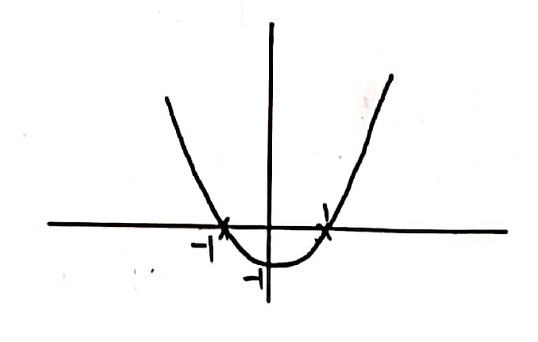
\includegraphics[width=1.8in,height=1.8in]{figures/ch08/figure1111_6.png}
	%\caption{This is an inserted JPG graphic} 
	%\label{fig:graph} 
	\end{marginfigure}
\end{enumerate}

%Above are notes for Nov 11